\documentclass[12pt]{report}

\usepackage[a4paper,width=150mm,top=25mm,bottom=25mm,bindingoffset=6mm]{geometry}
\usepackage[onehalfspacing]{setspace}
\usepackage{ucs}
\usepackage[table,xcdraw]{xcolor}
\definecolor{mColor1}{rgb}{0.9,0.9,0.9}

\usepackage{fancyhdr}
\pagestyle{fancy}
\fancyhead{}
\renewcommand{\chaptermark}[1]{\markboth{#1}{}}
\renewcommand\sectionmark[1]{\markright{\thesection\ #1}}

\fancyhead[LO, RE]{\leftmark}
\fancyhead[LE, RO]{\rightmark}

\usepackage{titlesec, blindtext, color}
\definecolor{gray75}{gray}{0.75}
\usepackage{mathptmx}
\usepackage[utf8]{inputenc}
\usepackage[T1]{fontenc}
\usepackage[ngerman]{babel}

\usepackage{amsmath,amssymb,amstext,amsthm,mathtools}
\usepackage{url}
\usepackage{caption}
%\usepackage[belowskip=-5pt,aboveskip=0pt]{caption}
\usepackage{subcaption}

\usepackage{float}
\usepackage{lscape}
\usepackage{pdfpages}
\usepackage{rotating}
\usepackage{graphicx}
\setlength\parindent{0pt}
\usepackage{hyperref}
\usepackage{acronym}
\usepackage{textcmds}
\usepackage{longtable}
\usepackage[export]{adjustbox}
\usepackage{upgreek}
\usepackage{dsfont}
\usepackage{tensor}
\usepackage{amsbsy}
\usepackage{multirow, hhline, colortbl}
\usepackage[table]{xcolor}


\DeclareMathAlphabet{\mathcal}{OMS}{cmsy}{m}{n}
\SetMathAlphabet{\mathcal}{bold}{OMS}{cmsy}{b}{n}

\usepackage{listings, lstautogobble}
\usepackage{textcomp}
\definecolor{yo}{rgb}{0.9,0.6,0}
\definecolor{Gray}{gray}{0.9}
\definecolor{listinggray}{gray}{0.9}
\definecolor{lbcolor}{rgb}{0.95,0.95,0.95}
\definecolor{greylines}{rgb}{0.9529,0.9529,0.9529}

\lstset{
	backgroundcolor=\color{lbcolor},
	tabsize=4,
	rulecolor=,
	language=python,
        basicstyle=\scriptsize,
        upquote=true,
        aboveskip={1.5\baselineskip},
        columns=fixed,
        showstringspaces=false,
        extendedchars=true,
        breaklines=true,
        prebreak = \raisebox{0ex}[0ex][0ex]{\ensuremath{\hookleftarrow}},
        frame=lines,
        showtabs=false,
        showspaces=false,
        showstringspaces=false,
        identifierstyle=\ttfamily,
        keywordstyle=\color[rgb]{0.55,0,0},
        alsoletter={/,*,[,]},%
        otherkeywords={},
        morekeywords=[2]{with, as},
        morekeywords=[3]{},
        emph={self},          % Custom highlighting
		emphstyle=\color[rgb]{0.1,0.3,1},
		emph={[2]f},          % Custom highlighting
		emphstyle={[2]\color[rgb]{0.1,0.5,0.1}},
		emph={[3]__init__},          % Custom highlighting
		emphstyle={[3]\color[rgb]{0.1,0.3,1}},
		emph={[4]open,str,print,KeyError},          % Custom highlighting
		emphstyle={[4]\color[rgb]{0.2,0.6,0.8}},
        commentstyle=\color[rgb]{0.3,0.3,0.3},
        stringstyle=\color[rgb]{0.133,0.545,0.133},
        	autogobble=true
}
\lstnewenvironment{ttlisting}{\lstset{basicstyle=\scriptsize}}{}

\usepackage{color}
\usepackage[section]{placeins}

\newenvironment{simplechar}{%
	\catcode`\$=12
	\catcode`\&=12
	\catcode`\#=12
	\catcode`\^=12
	\catcode`\_=12
	\catcode`\~=12
	\catcode`\%=12
	\catcode`\"=12
	\catcode`\'=12
	}{}{}

\newtheoremstyle{dotless}{}{}{\itshape}{}{\bfseries}{}{ }{}

\theoremstyle{dotless}

\newtheorem{thm}{Theorem}
\newtheorem{defn}[thm]{Definition}
\newtheorem{exmp}[thm]{Example}
\theoremstyle{definition}


\begin{document}

\begin{titlepage}
	Warum bin ich nicht einfach Staubsaugervertreter geworden?
\end{titlepage}

\tableofcontents

\chapter{Portfoliooptimierung}

\section{Nutzenoptimierung}

\subsection{Nutzenbasierte Portfoliooptimierung}

\subsubsection{Ausgangslage: Finanzpositionen}
\begin{itemize}
	\item Ein Investor hat das Ziel, ausgehend von einem Startkapital $v>0$, den Wert des Verm\"ogens zu einem Zeitpunkt $T$ zu optimieren
	\item Weitere Kapitalzuf\"uhrungen ider -entnahmen sind nicht vorgesehen
	\item Das Verm\"ogen $V$ zum Zeitpunkt $T$ kann mit einer reellwertigen Zufallsvariablen auf einem messbaren Raum identifiziert werden
	\item F\"ur Investitionen steht eine Menge $\mathcal{X}$ solcher Positionen zur Auswahl
\end{itemize}

\subsubsection{Pr\"aferenzordnung}

\begin{itemize}
	\item Die Pr\"aferenzordnung $\succ$ auf $\mathcal{X}$ sei \"uber das Pr\"aferenzfunktional $\mathcal{U}(X) = \mathbb{E_P}[x(X)]$ expliziert
	\item $X \succ Y \Leftrightarrow \mathbb{E_P}[x(X)] > \mathbb{E_P}[x(Y)]$, $(X,Y \in \mathcal{X})$
	\item $\mathbb{P}$ ein Referenzwahrscheinlichkeitsma{\ss}
	\item $u$ eine Nutzenfunktion
	\item Annahme: risikoaverses Verhalten der Investoren
	\item Nutzenfunktion einer risikoaversen Person: $u:S \subset \mathbb{R} \rightarrow \mathbb{R} \cup \{\infty\}, \ x \rightarrow x(x)$, falls $u$ strikt konkav und strikt wachsend auf $S$
	\item Um die Positionen in $\mathcal{X}$ zu realisieren kann der Investor:
	\begin{itemize}
		\item geeignete Portfolios aus prim\"aren Finanzprodukten konstruieren
		\item mit derivaten Produkten handeln
	\end{itemize}
	\item vollst\"andiger Markt: gleiche Menge erreichbarer Positionen mit beiden F\"allen
	\item unvollst\"andiger Markt: Derivate bieten mehr Flexibilit\"at
\end{itemize}



\section{Portfoliotheorie nach Markowitz}

\subsection{Grundlagen}

\begin{itemize}
	\item Ausgangspunkt: Universum aus $n$ Finanztiteln
	\item Risikoebene: Diversifikation
	\item Risiko/Wert-Ebene: Rendite/Risiko-Dominanz und effiziente Portfolios
	\item Ein Portfolio mit Rendite $R_1$ dominiert ein Portfolio mit Rendite $R_2$, wenn entweder \\ $Var(R_1) < Var(R_2)$ und $\mathbb{E}[R_1] \geq \mathbb{E}[R_2]$ \\ oder \\ $\mathbb{E}[R_1] > \mathbb{E}[R_2]$ und $Var(R_1) \leq Var(R_2)$
	\item Portfolio EV-effizient, wenn es durch kein anderes Portfolio dominiert wird
	\item nur effiziente Portfolios k\"onnen optimale Portfolios sein
\end{itemize}

\begin{figure}[H]
\centering
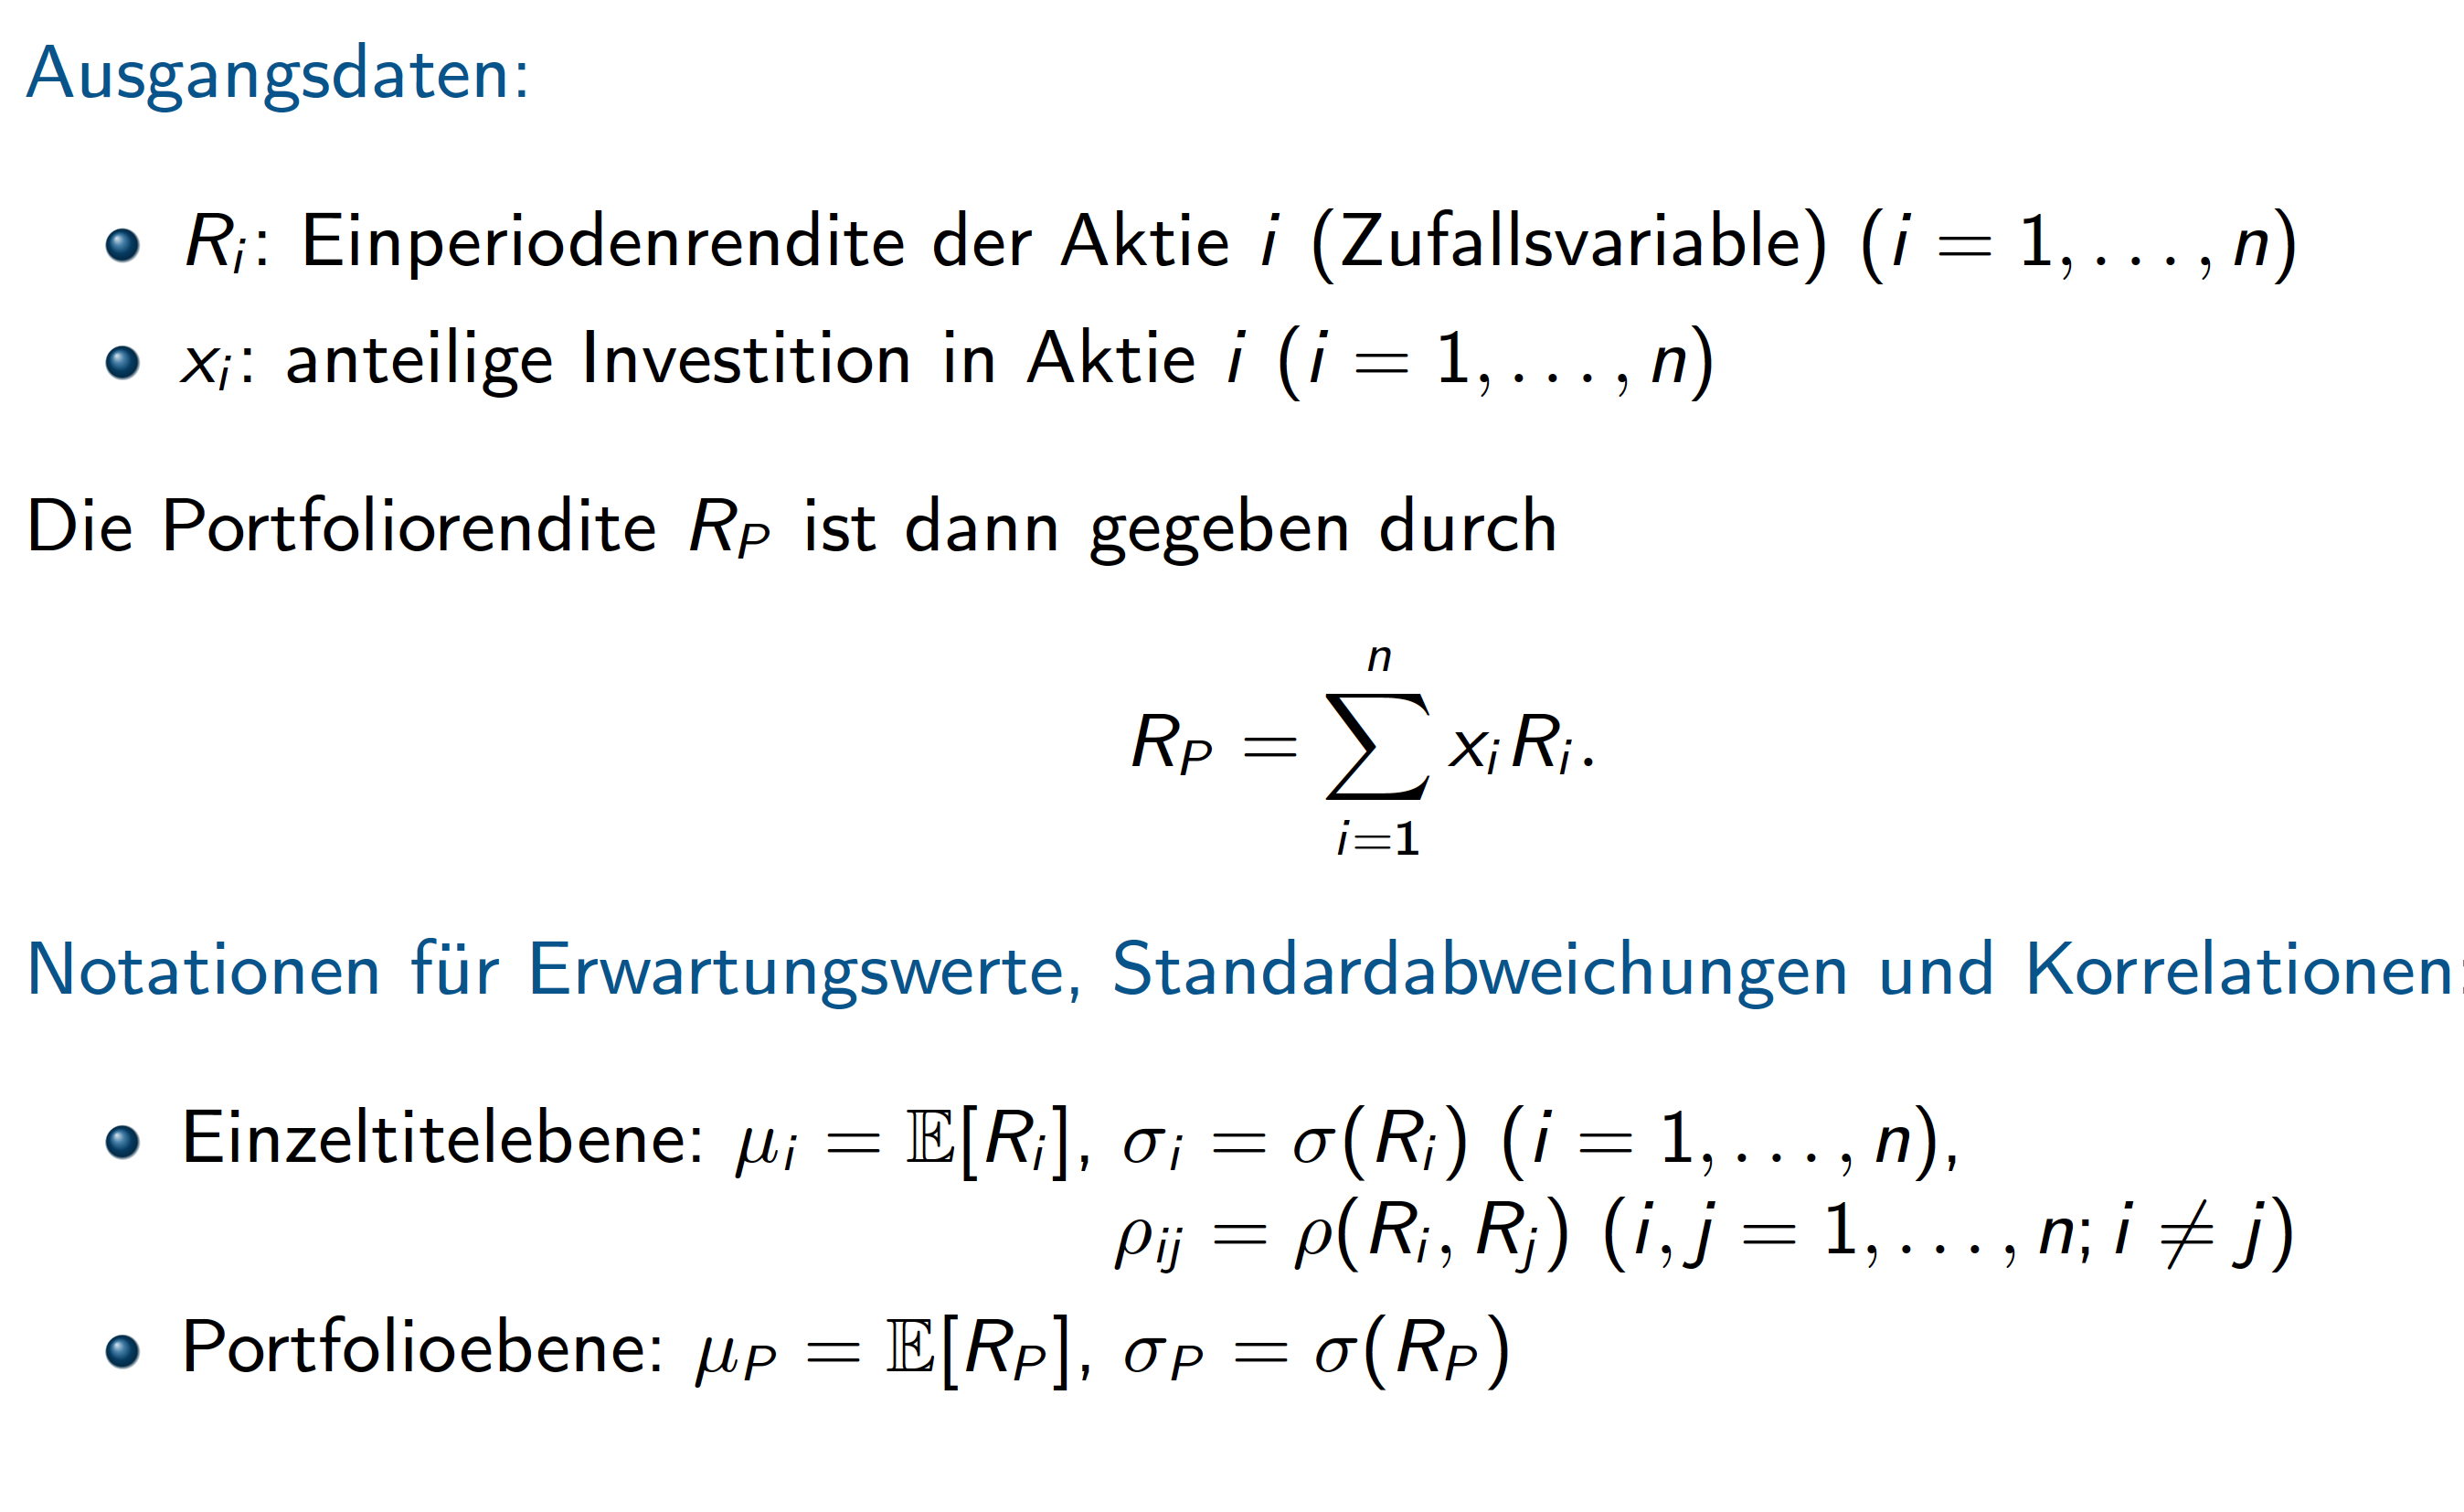
\includegraphics[width=\textwidth]{Bilder/Ausgangsdaten.png}
\end{figure}

\subsection{Effiziente Portfolios}

\begin{figure}[H]
\centering
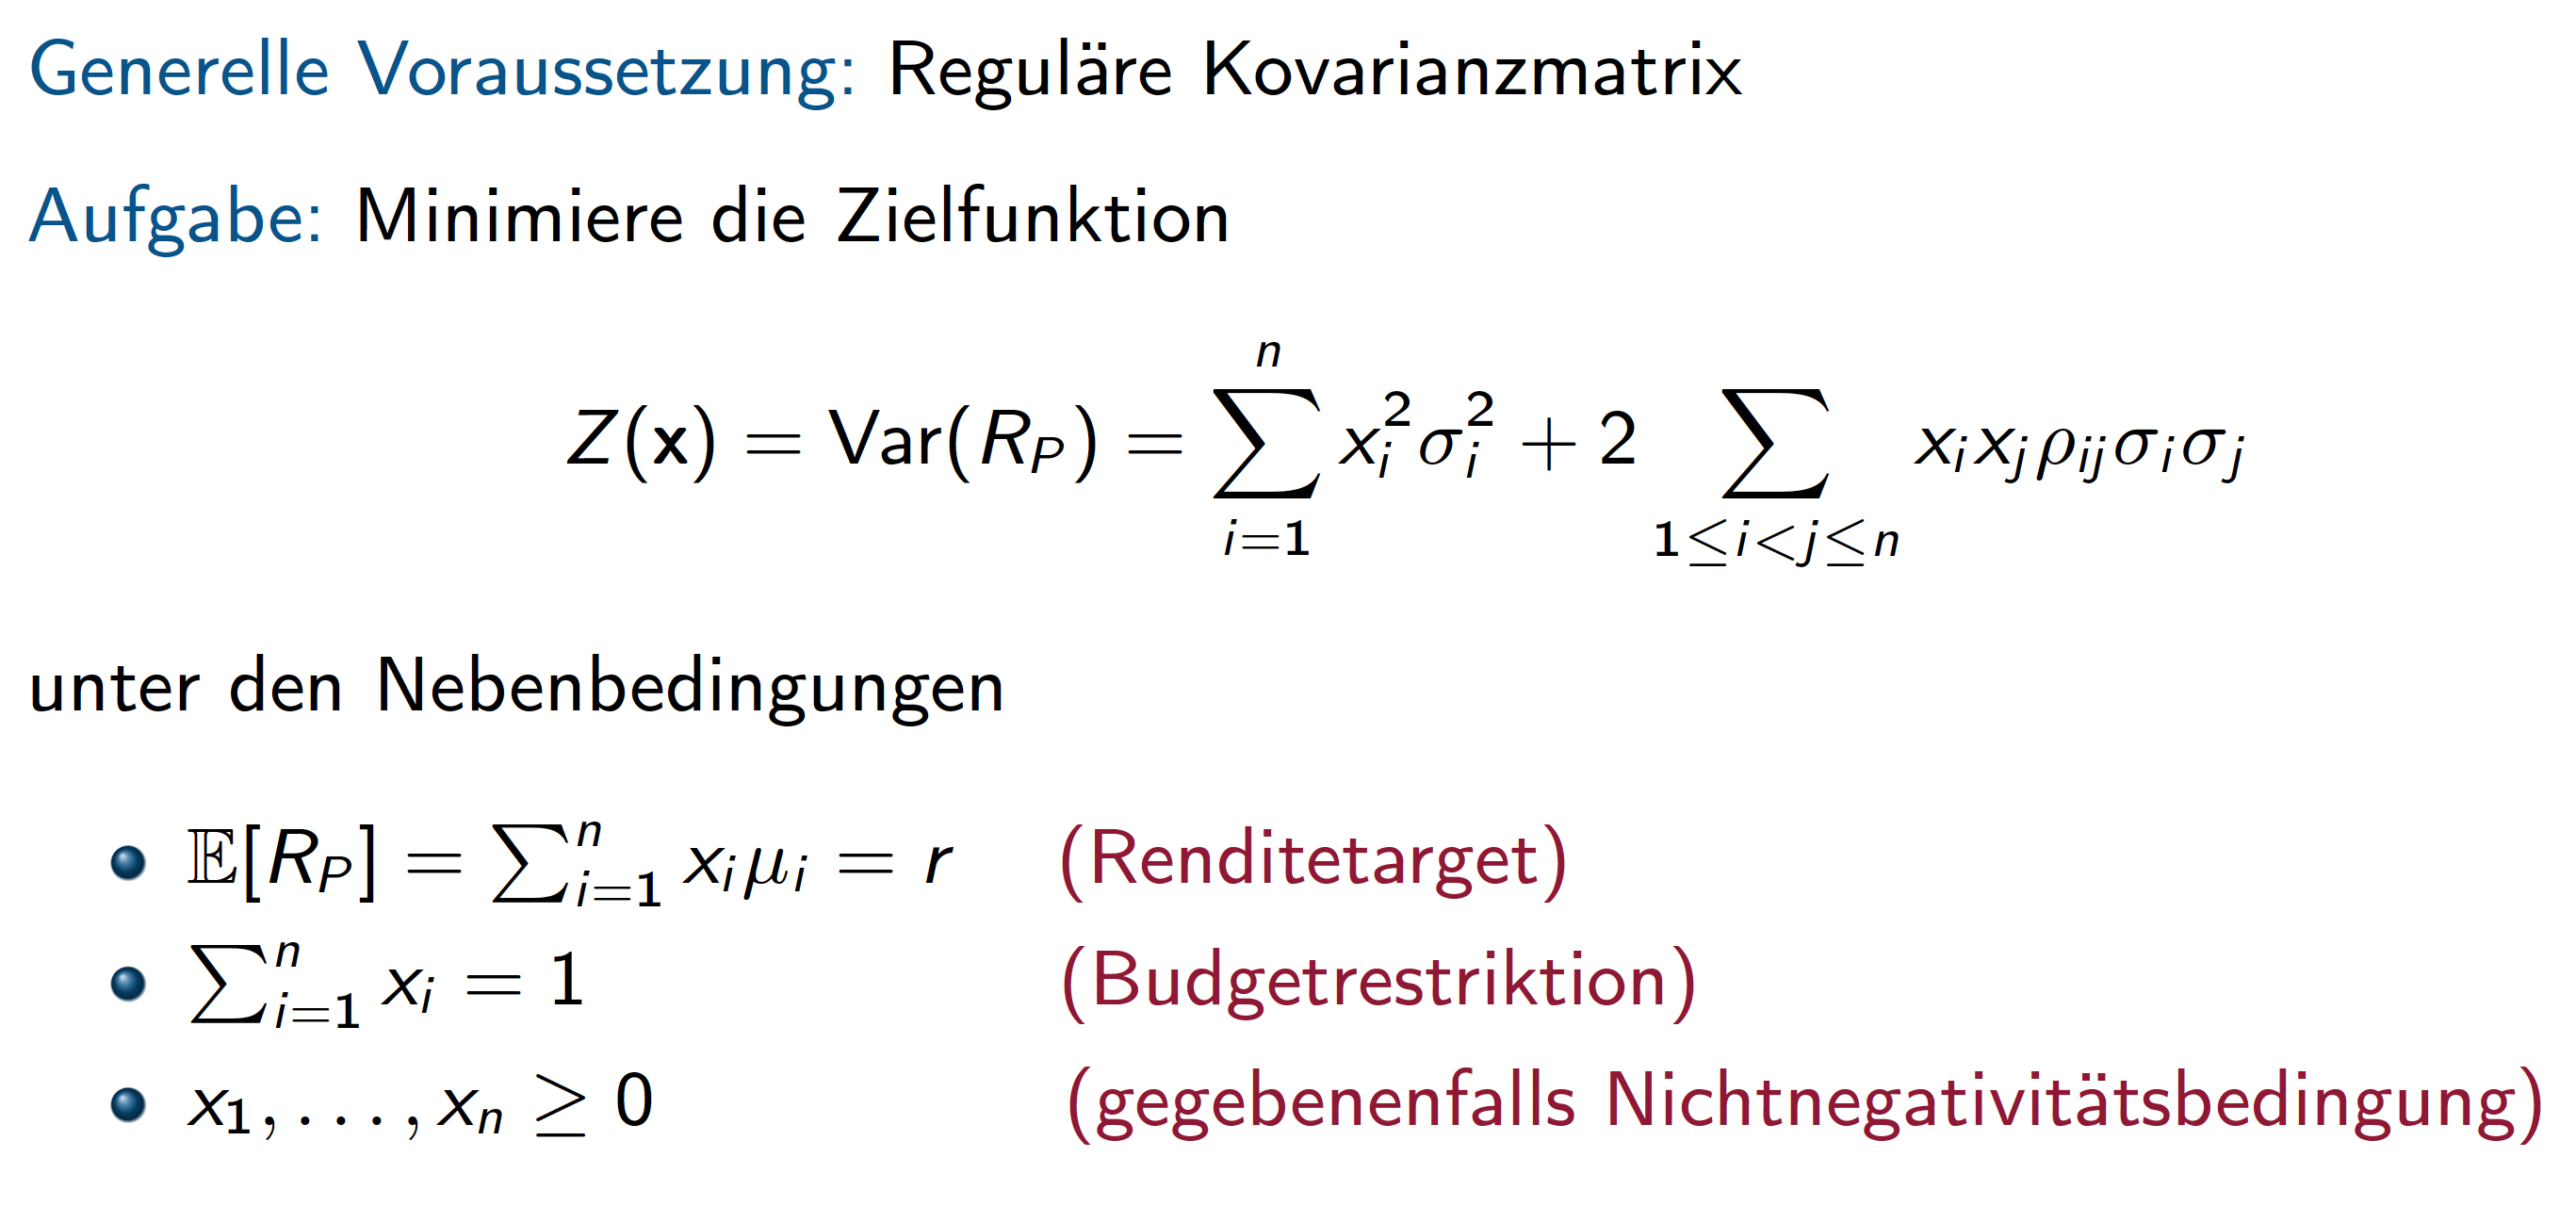
\includegraphics[width=\textwidth]{Bilder/Minimierungsproblem.png}
\end{figure}

\begin{itemize}
	\item Fall 1: Short Sales Allowed, L\"osung mit Lagrange-Ansatz, lokalen Extremwert der Lagrange-Funktion bestimmen
	\begin{itemize}
		\item geometrischer Rand der Menge aller zul\"assigen Portfolios besteht aus den Punkten, die bez\"uglich eines fixierten Erwartungswerts eine minimale Varianz aufweisen
		\item geometrischer Rand ist eine Wurzelfunktion (als Funktion von $\sigma^2$, bzw. der rechte Ast der Hyperbel (als Funktion von $\sigma^2$
		\item der effiziente Rand entspricht dem oberen Ast der Kurve inklusive dem global varianzminimalen Portfolio
	\end{itemize}
	\item Fall 2: No Short Sales, Quadratische Programmierung, i.A. keine analytische L\"osung, numerische Verfahren
\end{itemize}

\subsubsection{Alternative Formulierungen des Problems}

\begin{figure}[H]
\centering
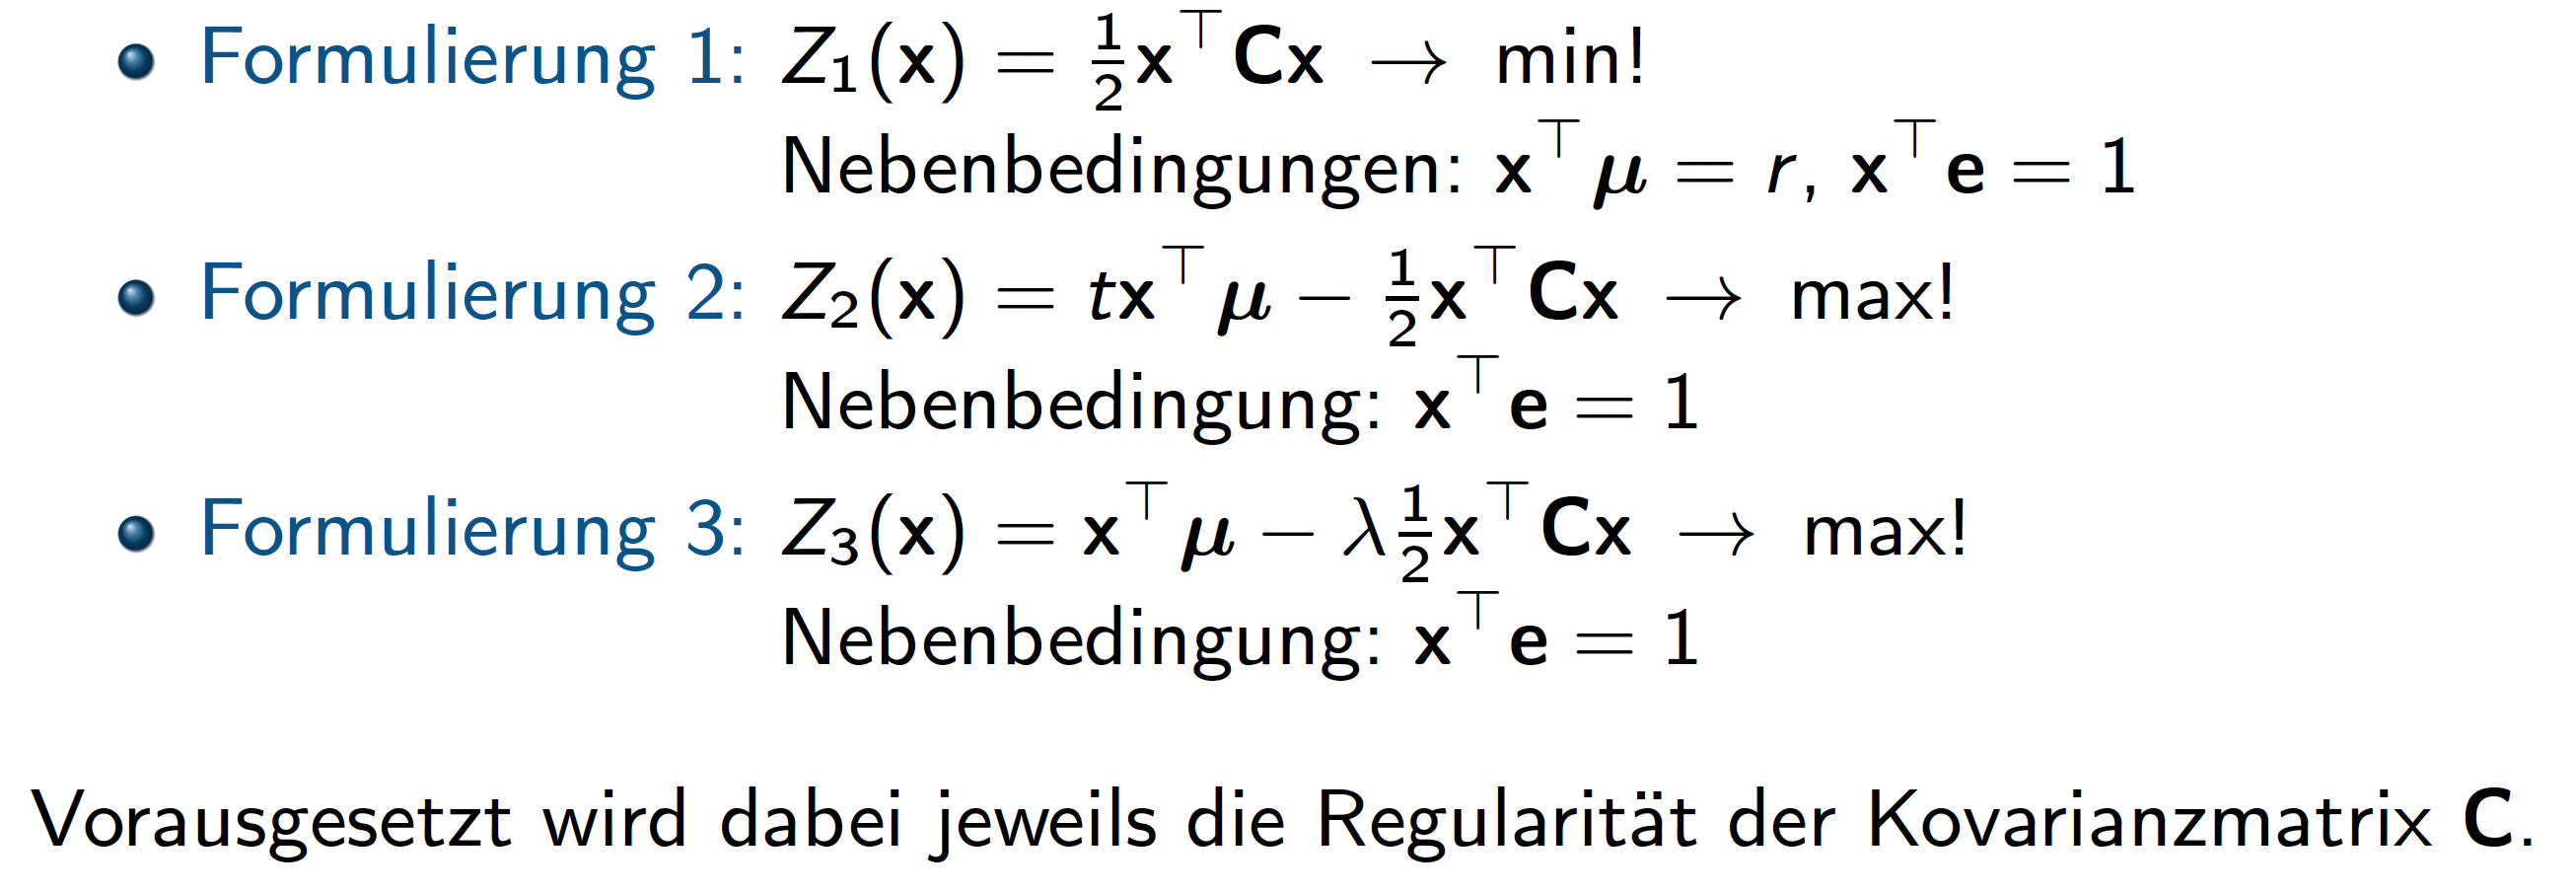
\includegraphics[width=\textwidth]{Bilder/alternativeFormulierungen.png}
\end{figure}

\begin{itemize}
	\item Lagrange-Funktion f\"ur Formulierung 2: \\ $L(x, \lambda) = tx^T \mu - \frac{1}{2} x^T Cx - \lambda (x^T e - 1)$ 
	\item $\sigma^2 = \sigma_0^2 + \frac{1}{\alpha_1}(\mu - \mu_0)^2$
	\item $\mu = \mu_0 \pm \sqrt{\alpha_1 (\sigma^2 - \sigma_0^2) }$
\end{itemize}



\subsection{Portfolioselektion}

\begin{itemize}
	\item Trade-Off zwischen Risiko und Rendite, d.h. Selektion einer charakteristischen $(\sigma, \mu)$-Position auf dem effizienten Rand
	\item Spezifizierung einer EV-Pr\"aferenzfunktion: $\mathcal{U}(R)=H(\mathbb{E}[R], \sigma(R))$
	\item Optimierungsproblem: $H(\mu, \sigma) = V(x_1,...,x_n) \rightarrow max$, Nebenbed.: $(\sigma, \mu) \in M, (x_1,...,x_n) \in D$ mit M Menge der zul\"assigen $(\mu, \sigma)$-Positionen bzw. $D$ die Menge der zul\"assigen Investmentgewichte
\end{itemize}

\subsection{Probleme des Markowitz-Ansatzes}

\begin{itemize}
	\item Markowitz-Basismodell beruht auf Risikoma{\ss} Standardabweichung (vor allem f\"ur symmetrische Verteilungen, in der Praxis aber oft signifikante Schiefe vorhanden)
	\item Optimierte Portfolios besitzen oftmals extreme Allokationen (hohe Leerverkaufspositionen oder geringe Diversifikation, optimale Portfolios \"ubergewichten Assets, die hohe gesch\"atzte erwartete Renditen und geringe Varianzen aufweisen)
	\item Optimierung sehr sensitiv bez\"uglich Inputdaten
\end{itemize}

\section{Alternative Ans\"atze der Portfoliooptimierung}

\begin{itemize}
	\item Markowitz-Modell: Standardabweichung als Risikoma{\ss}
	\item jetzt andere Risikoma{\ss}e verwenden
	\item Value at Risk:
	\begin{itemize}
		\item nicht subadditiv
		\item Portfoliorisiko $V@R_{\lambda}(R_P(x))$ i.A. keine konvexe Funktion
	\end{itemize}
	\item Average Value at Risk
	\begin{itemize}
		\item lageabh\"angiges Risikoma{\ss} (auch Mean-AV@R und Mean-V@R in der Literatur betrachtet)
		\item Generelle Form: $AV@R_{\lambda}(R_P(x)) \rightarrow min$
		\item Nebenbedingungen:
		\item[1.] $E[R_P(x)] = r$
		\item[2.] $x^Te = 1$
		\item[3.] $x \geq 0$ 
		\item $AV@R_{\lambda}(X) = V@R_{\lambda}(X) + \frac{1}{\lambda} \mathbb{E}[(-X-V@R_{\lambda}(X))^{+}]$
	\end{itemize}
\end{itemize}

\section{Asset Pricing}

\subsection{Portfoliotheorie mit sicherer Anlage}

\subsubsection{Erweiterung des Anlagespektrums}
\begin{itemize}
	\item Risikolose Anlage (Renditevarianz = 0) zum sicheren Zins $r_0$
	\item vollkommener Kapitalmarkt: zum Zins $r_0$ k\"onnen beliebige Betr\"age angelegt oder aufgenommen werden
\end{itemize}

\subsubsection{Elementare Analyse}
\begin{itemize}
	\item fixiere riskantes Portfolio $P \in M$, d.h. Portfolio aus der Menge der durch Aktienmischung realisierbaren Portfolios
	\item Betrachte Portfolio, das z.T. in sichere Anlagen investiert und zum Teil in $P$
	\item $R_P$ ist die Rendite von $P$
	\item $0 \leq x \leq \infty$ anteilige Investition in $P$
	\item $-\infty < 1-x \leq 1$ anteilige in Investition in sichere Anlage
	\item Rendite gesamt: $R=xR_P + (1-x)r_0$
	\item $\mu = r_0+x(\mu_P - r_0)$
	\item $\sigma^2 = x^2 \sigma_P^2$
	\item[$\Rightarrow$] $\mu = r_0 + \frac{\mu_P-r_0}{\sigma_P}\sigma$
	\item Menge aller effizienten bzw. optimalen Portfolios ist eine Gerade (Tangentialgerade an den bisherigen effizienten Rand 
\end{itemize}

\subsection{Capital Asset Pricing Model}

\subsubsection{Pr\"amissen des CAPM}
\begin{itemize}
	\item Fall $r_0 < \mu_0$
	\item Es gibt $m$ EV-Investoren mit Wertpapierbudgets $V_i >0$, $V = \sum_{i=1}^m V_i$
	\item alle Investoren sch\"atzen $r_0$, $\mathbb{E}[R_i]$, $Var(R_i)$ und $Cov(R_i,R_j)$ gleich ein
	\item Marktgleichgewicht (Angebot = Nachfrage)
\end{itemize}

\subsubsection{Marktportfolio}
\begin{itemize}
	\item jeder Investor erwirbt EV-effizientes Portfolio, Anteil $\lambda_i$ des Budgets $V_i$ in Tangentialportfolio, Rest ($1-\lambda_i$) in sichere Anlage
	\item Nachfrageportfolio des Marktes nach Aktien: $(\lambda^T V)x_T$
	\item Angebotsportfolio: alle Aktien, die zu $t=0$ zu Marktwerten bewertet werden
\end{itemize}

\begin{figure}[H]
\centering
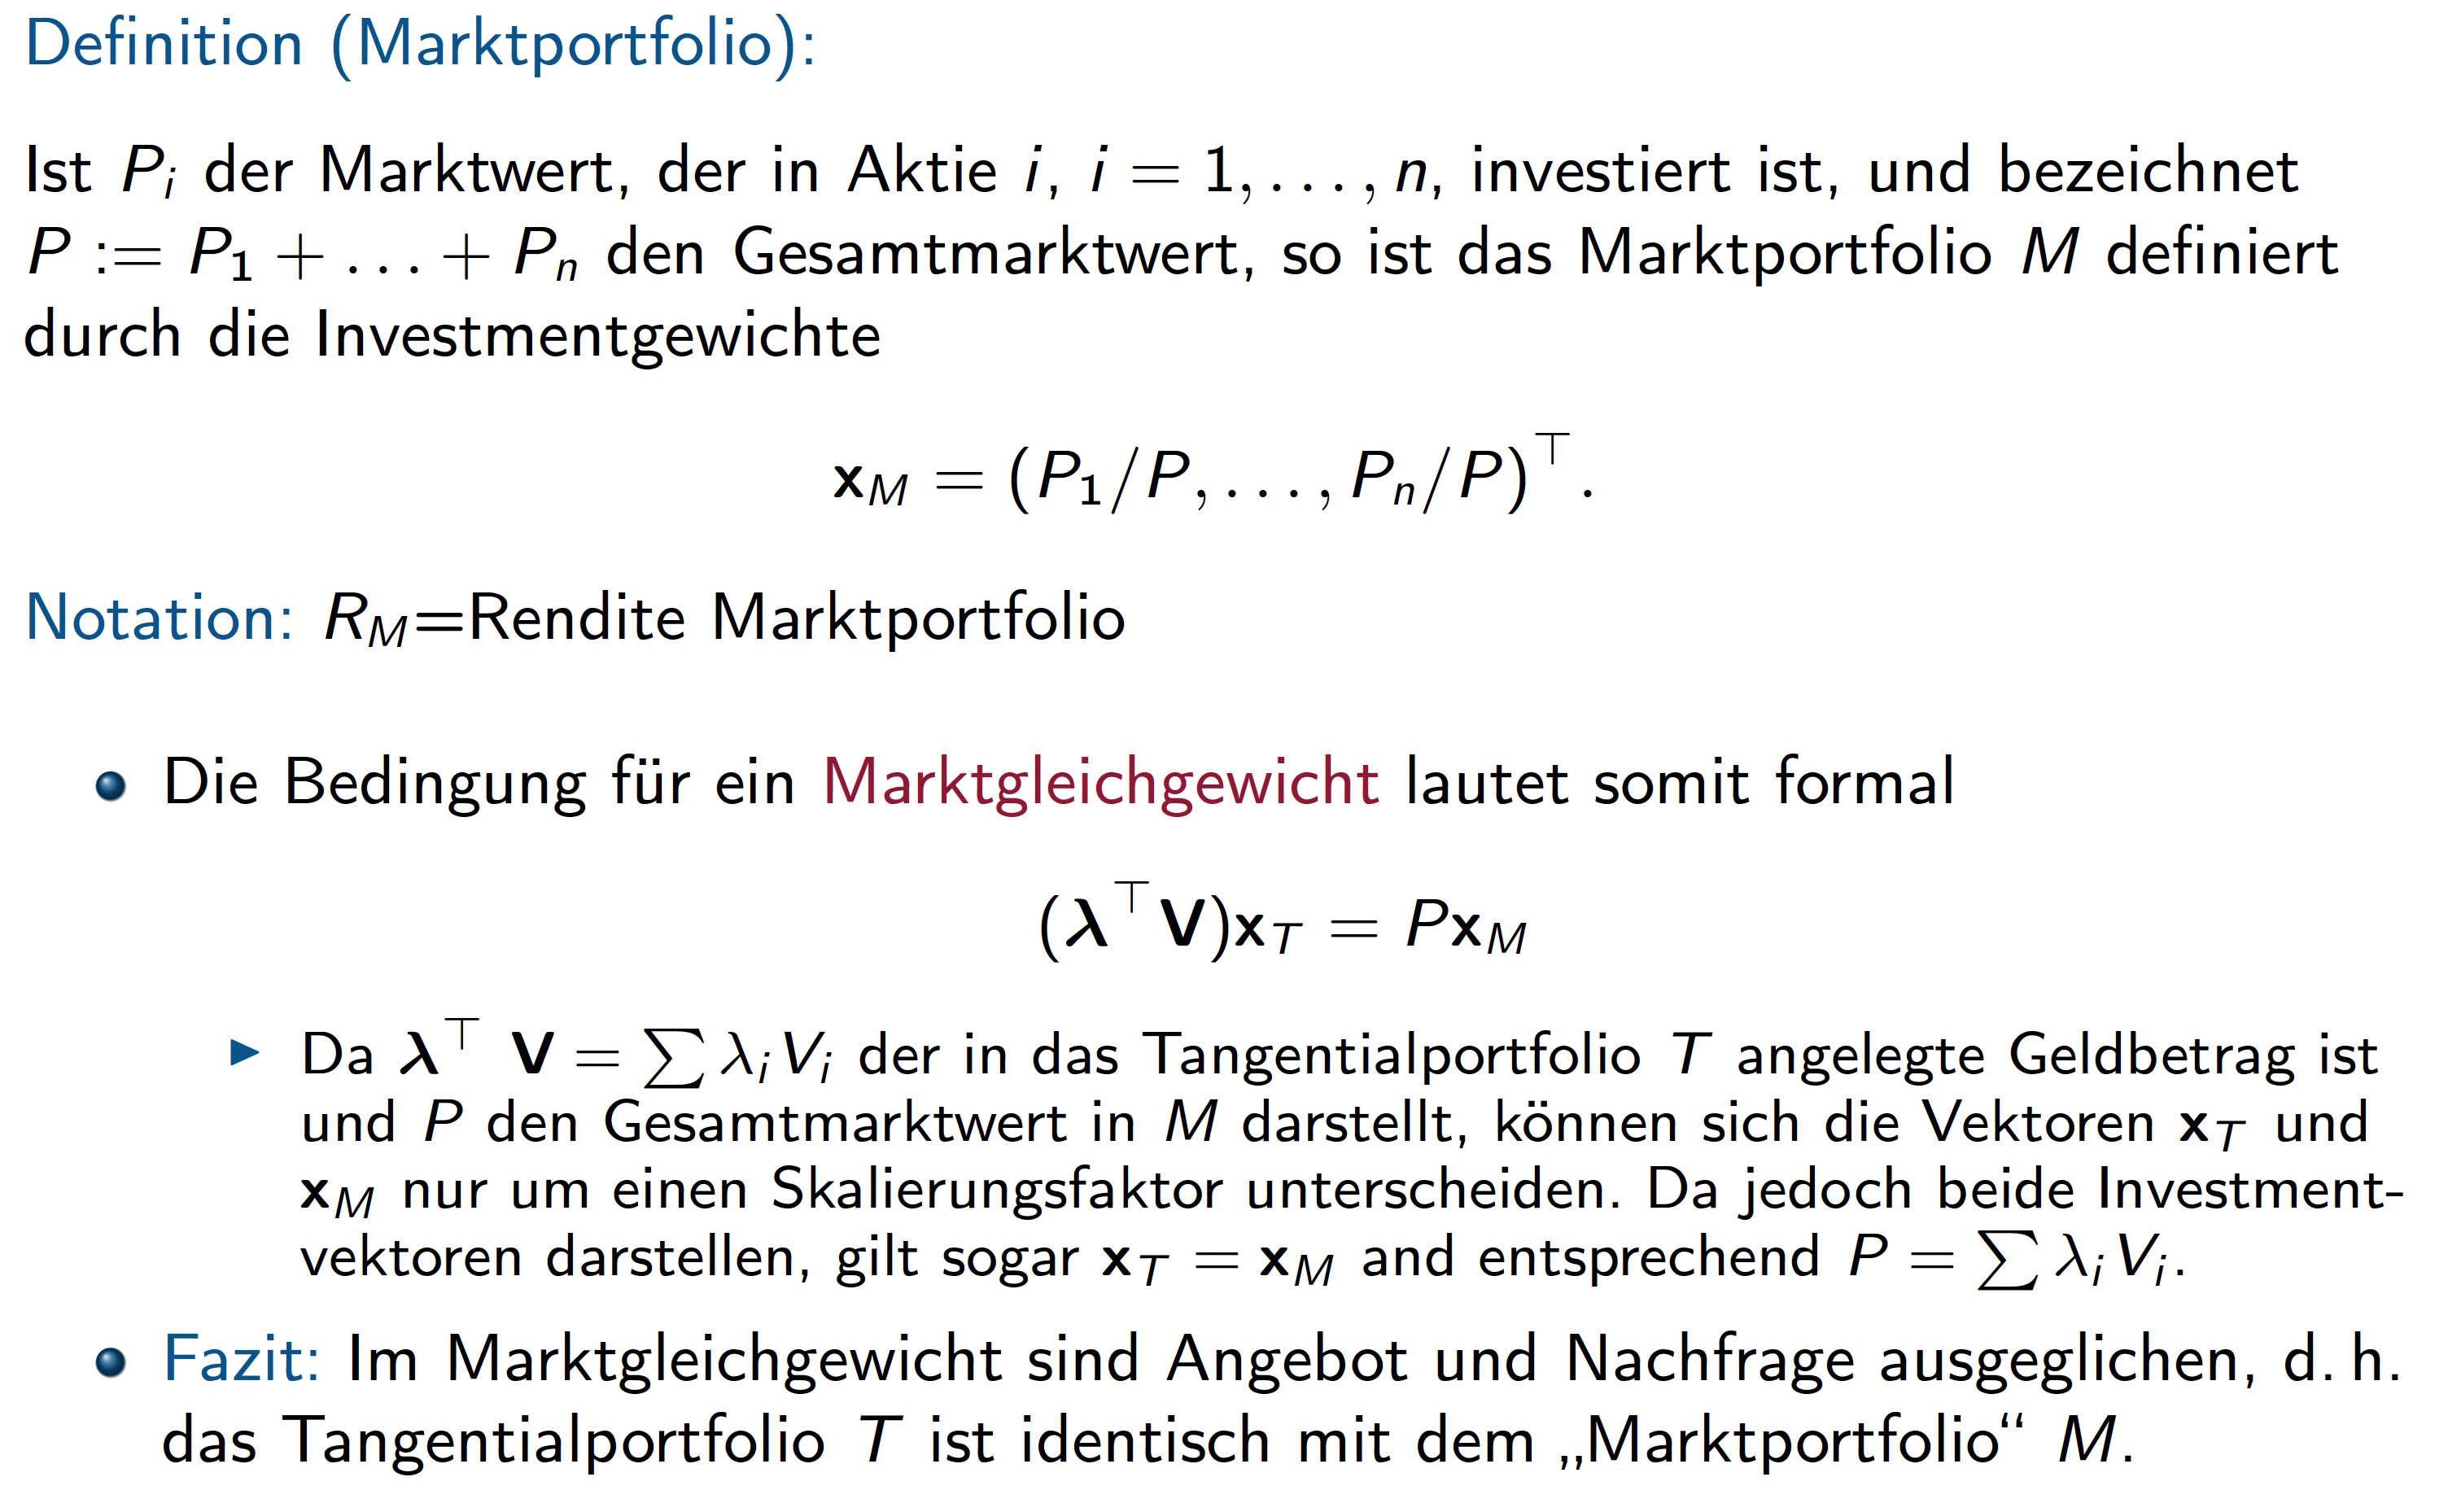
\includegraphics[width=\textwidth]{Bilder/Marktportfolio.png}
\end{figure}

\subsubsection{CAPM-Analytik}

\begin{figure}[H]
\centering
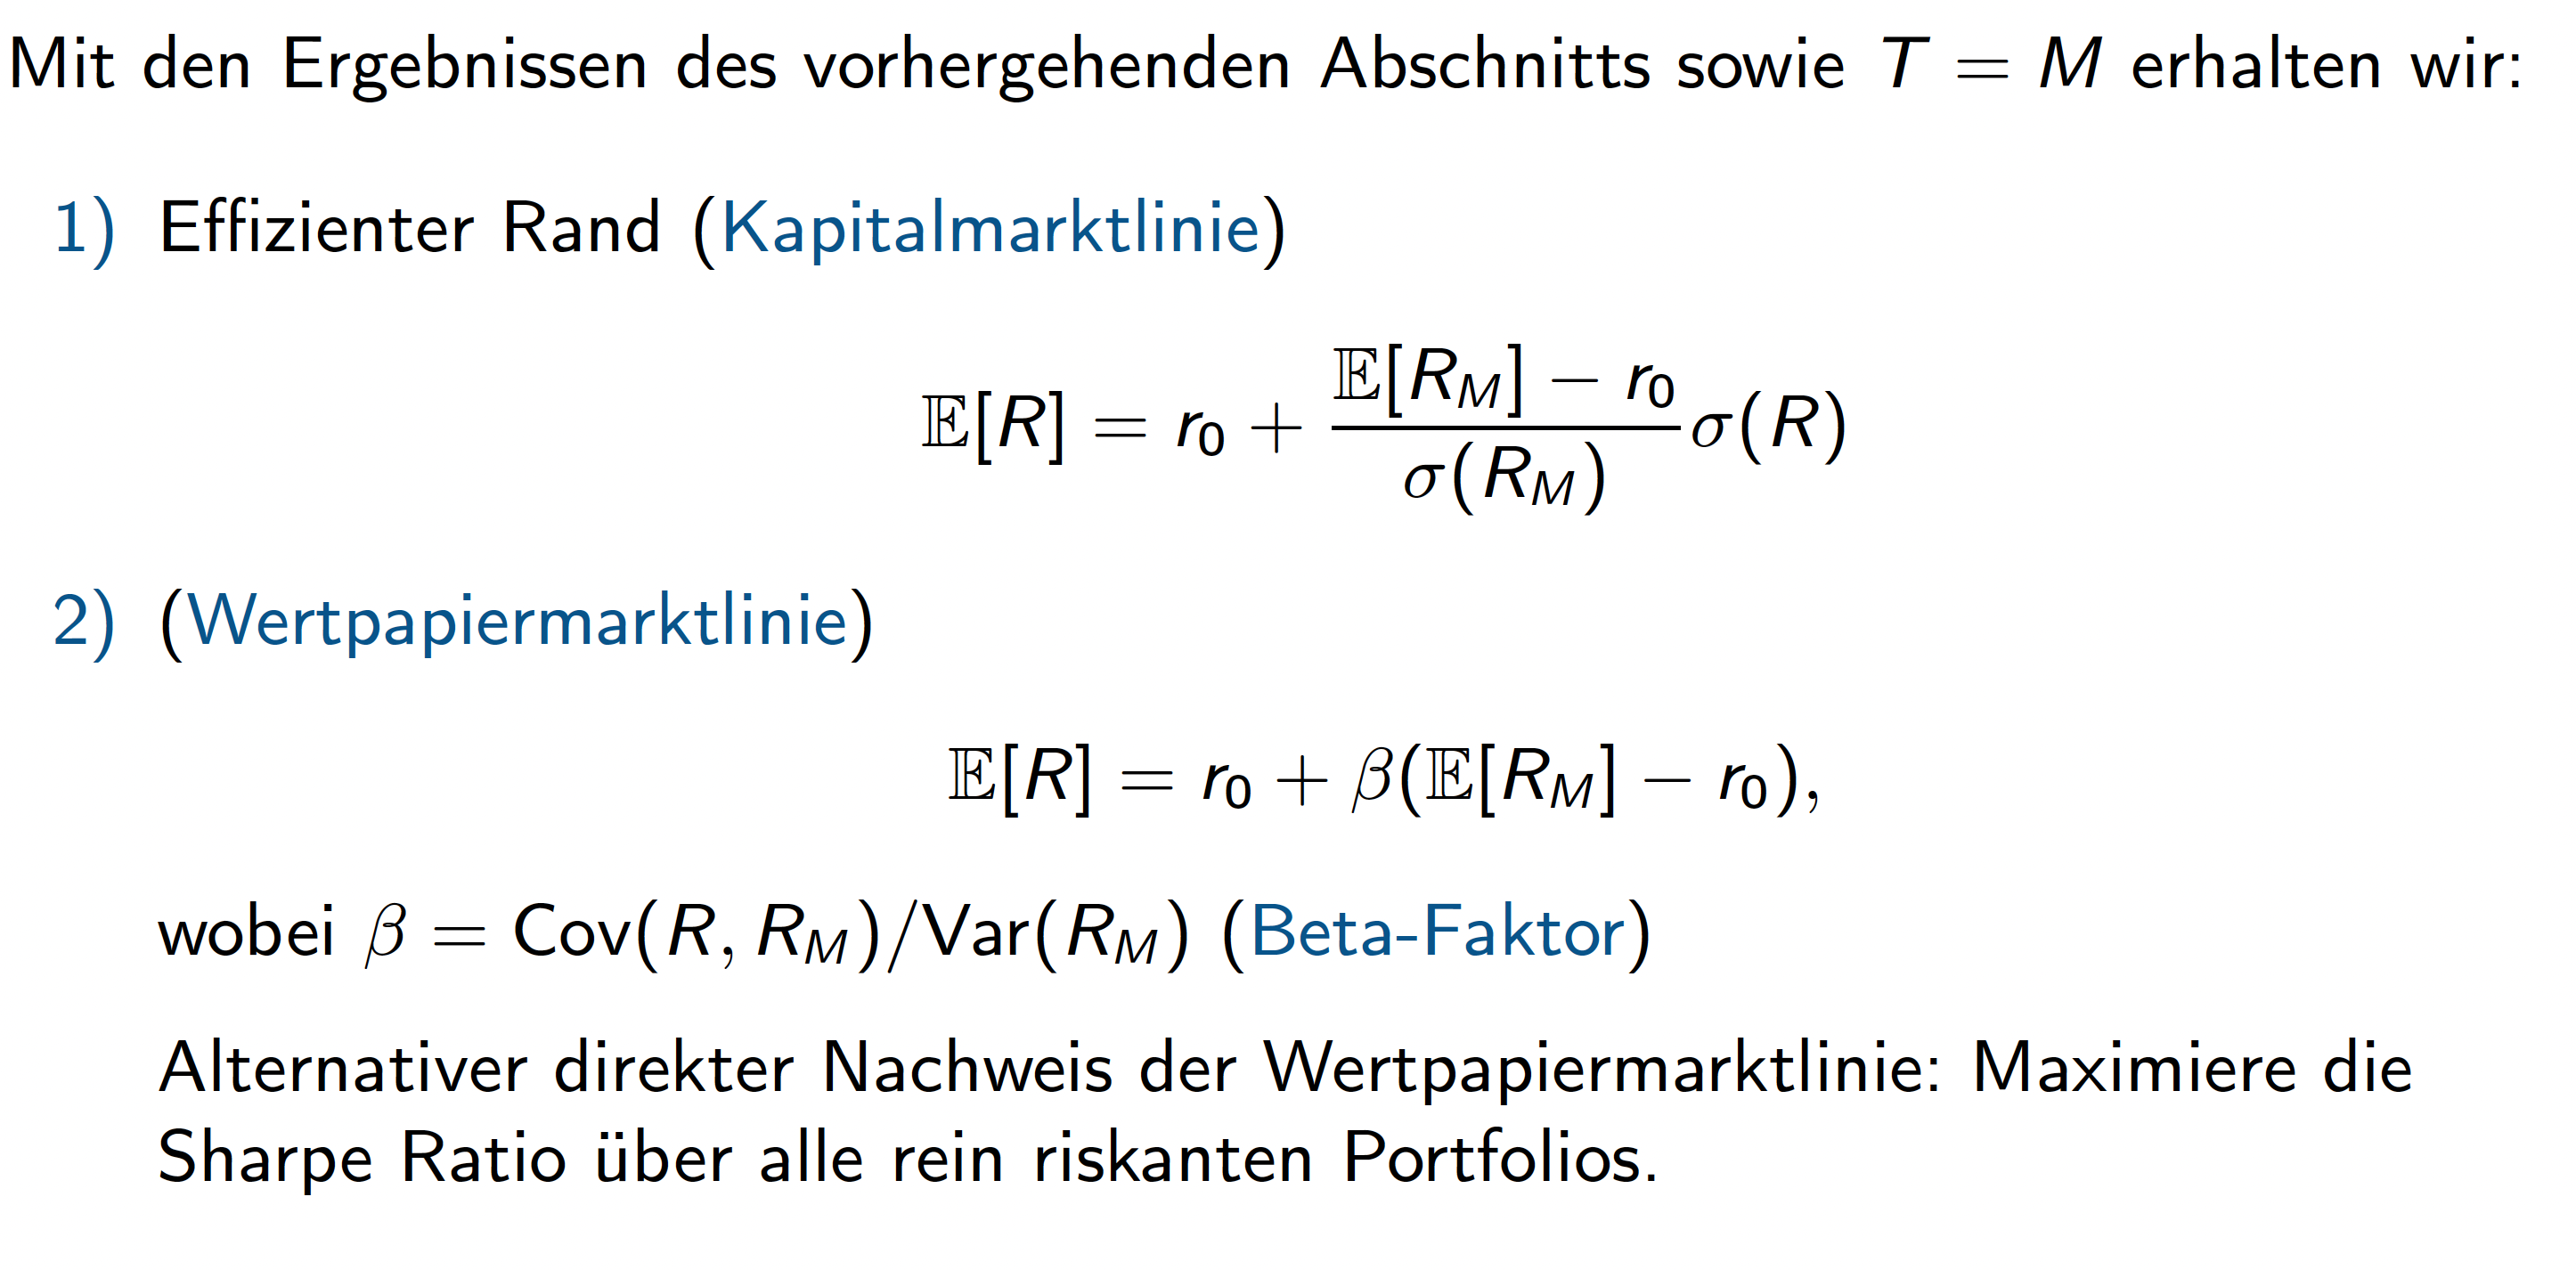
\includegraphics[width=\textwidth]{Bilder/CAPMAnalytik.png}
\end{figure}

\subsubsection{Hauptresultate des CAPM}

\begin{itemize}
	\item Menge aller optimalen Portfolios $R$ (Kapitalmarktlinie): $\mathbb{E}[R] = r_0 + \frac{\mathbb{E}[R_M] - r_0}{\sigma(R_M)}\sigma(R)$
	\item Menge aller optimalen Portfolios $R$ (Wertpapiermarktlinie): $\mathbb{E}[R] = r_0 + \beta_R(\mathbb{E}[R_M] - r_0)$ mit $\beta_R = \frac{Cov(R,R_M)}{Var(R_M)}$
	\item Preisgleichung $P= \frac{\mathbb{E}[V]}{1+r_0+\beta(\mathbb{E}[R_M]-r_0)}$ 
	\item $P$ der anf\"anglichen Preisen eines Titels mit zufallsabh\"angigem Endwert $V$ und korrespondierender Einperiodenrendite $R$
	\item $r_0$ sicherer Zins
	\item $R_M$ Rendite des Marktportfolios
\end{itemize}









































































\end{document}
